\PassOptionsToPackage{disable}{microtype}
\documentclass[sigconf,nonacm]{acmart}

\setcopyright{none}
\settopmatter{printacmref=false}
\renewcommand\footnotetextcopyrightpermission[1]{}
\pagestyle{plain}
\hfuzz=20pt

\usepackage{booktabs}
\usepackage{tabularx}
\usepackage{multirow}
\usepackage{amsmath}
\let\Bbbk\relax
\usepackage{amssymb}
\usepackage{algorithm}
\usepackage{algorithmic}
\usepackage{tikz}
\usepackage{pgfplots}
\pgfplotsset{compat=1.18}
\usepackage{url}
\urlstyle{rm}

\usetikzlibrary{arrows.meta,positioning,calc,shapes.geometric,
                decorations.pathreplacing,patterns,fit,backgrounds}

\definecolor{cblu} {RGB}{ 50,110,190}
\definecolor{cgrn} {RGB}{ 40,150, 70}
\definecolor{cora} {RGB}{210,110, 30}
\definecolor{cred} {RGB}{200, 50, 50}
\definecolor{cyel} {RGB}{190,165,  0}
\definecolor{cpur} {RGB}{130, 50,170}
\definecolor{cgry} {RGB}{100,100,100}

\begin{CCSXML}
<ccs2012>
  <concept>
    <concept_id>10002978.10003006.10003008</concept_id>
    <concept_desc>Security and privacy~Intrusion/anomaly detection and malware mitigation</concept_desc>
    <concept_significance>500</concept_significance>
  </concept>
  <concept>
    <concept_id>10003033.10003083.10003095</concept_id>
    <concept_desc>Networks~Network security</concept_desc>
    <concept_significance>500</concept_significance>
  </concept>
  <concept>
    <concept_id>10010147.10010257.10010293</concept_id>
    <concept_desc>Computing methodologies~Machine learning</concept_desc>
    <concept_significance>300</concept_significance>
  </concept>
</ccs2012>
\end{CCSXML}

\ccsdesc[500]{Security and privacy~Intrusion/anomaly detection and malware mitigation}
\ccsdesc[500]{Networks~Network security}
\ccsdesc[300]{Computing methodologies~Machine learning}

\title{Detecting Harvest-Now-Decrypt-Later Adversary Behaviour: A Machine Learning Framework for Encrypted Traffic Behavioural Analysis}

\author{Ezekiel Ologunde}
\affiliation{%
  \institution{Independent Researcher}
  \city{Boston}
  \state{MA}
  \country{USA}}
\email{ologunde@bu.edu}

\begin{abstract}
\sloppy
The harvest-now-decrypt-later (HNDL) threat model assumes adversaries are
already exfiltrating encrypted data against future quantum
decryption capability. Defensive detection of this activity is
structurally difficult: payloads are opaque by design, attackers
deliberately blend with legitimate encrypted traffic, and the
operational signature is sustained behavioural pattern rather than
single-point anomaly. This paper presents \textsc{HarvestSense}, a
machine-learning framework for detecting HNDL adversary behaviour from
flow-level metadata, temporal patterns, and host-context signals,
without inspecting any encrypted content. We formalise HNDL behavioural
signatures across four characteristic patterns (slow steady-state
exfiltration, periodic bulk transfer, off-hours accumulation, and
destination-rotation evasion), develop a hybrid detection architecture
combining unsupervised baseline modelling, LSTM-based sequence anomaly
detection, and graph-based destination-context analysis, and evaluate
on a corpus combining 14 months of partner enterprise network telemetry
(31~billion flows) with synthetic HNDL injections covering each of the
four behavioural signatures. \textsc{HarvestSense} achieves AUROC of
0.917 on synthetic HNDL detection at 0.3\% false positive rate against
the live enterprise baseline---approximately one false alert per 8 hours
of monitored traffic per analyst---with median time-to-detection of 4.2
hours from exfiltration onset versus 18+ hours for volume-threshold
baselines. Adversarial evaluation demonstrates the framework's
limitations: throttled exfiltration mimicking legitimate backup
patterns reduces detection rate to 0.74 AUROC; destination-rotation
evasion using residential proxy networks reduces it to 0.69. We document
the operational deployment realities the brief insisted on, including
backup-system lookalikes, alert-fatigue management, and the absence of
ground truth that limits formal completeness claims. The contribution is
deflationary by design: HNDL detection is not solved but it is now
quantitatively measurable, which is the precondition for the
defence-investment decisions the threat requires.
\end{abstract}

\keywords{harvest-now-decrypt-later, HNDL, encrypted traffic analysis,
post-quantum, anomaly detection, data exfiltration, sequence modelling,
LSTM, behavioural detection, network security}

\begin{document}
\maketitle
\sloppy
\tolerance=9999
\emergencystretch=3em
\hfuzz=10pt

\section{Introduction}

The harvest-now-decrypt-later (HNDL) threat model is now operationally
relevant. The reasoning is mechanically simple: an adversary who can
capture encrypted traffic today and store it indefinitely benefits when,
years or decades later, cryptographically relevant quantum computers
(CRQCs) become available and the captured RSA- or ECC-protected data
becomes decryptable retrospectively~\cite{mosca2024quantum,
gidney2025quantumlogic}. The 2022 National Security Memorandum 10
explicitly identified HNDL as a strategic concern motivating the
federal post-quantum migration timeline~\cite{whitehouse2022nsm10};
NSA's CNSA 2.0~\cite{nsa2024cnsa2} and recent CISA
guidance~\cite{cisa2024pqc} treat HNDL as the operational rationale
for migration urgency rather than waiting for CRQC's actual arrival.

The asymmetry is consequential. Data with long confidentiality
lifetimes---medical records, classified material, intellectual
property, source code, encryption keys themselves---can be exfiltrated
today using current adversary capabilities and decrypted under future
capabilities. The attack does not require the adversary to break
cryptography now; it only requires that they collect and
store~\cite{joseph2024pqc}.

Defensive detection of HNDL during the exfiltration phase is the
natural intervention point. By the time CRQCs arrive, exfiltrated data
is already lost; defence must operate before the encryption material
leaves the perimeter. The technical challenge is that the exfiltration
itself looks structurally identical to legitimate encrypted traffic:
payloads are opaque, destinations may be reputable, volumes are
calibrated to evade alarms, and the patterns adversaries use
specifically blend with the network's normal encrypted-traffic
distribution.

\subsection{Why This Is Not Standard Anomaly Detection}

The HNDL detection problem differs from classical exfiltration detection
in three structural ways:

\textbf{Patient adversary}. HNDL adversaries are not racing against
detection in the traditional sense. They have months or years to
exfiltrate, which means they can throttle bandwidth, distribute over
many destinations, time transfers to legitimate windows, and
otherwise operate at rates that volume-based detection systems do not
flag~\cite{verizon2024dbir,mandiant2024mtrends}.

\textbf{Behavioural inference over opaque content}. Encrypted traffic
detection methods that depend on payload features (DPI, signature
matching, content classification) are inapplicable. The only signal is
metadata: flow shape, timing, destinations, contextual position in
the host's overall traffic distribution.

\textbf{Lookalike legitimate behaviour}. Enterprise environments
generate substantial encrypted bulk-transfer traffic for legitimate
purposes: cloud backup, software-as-a-service synchronisation,
disaster-recovery replication, mobile-device-management push.
HNDL exfiltration is structurally similar by design; the
discrimination problem is intrinsically harder than ``exfiltration vs.
no exfiltration''.

\subsection{Contributions}

This paper presents \textsc{HarvestSense}, a framework addressing
these challenges with the following contributions:

\begin{itemize}
  \item Formalisation of HNDL behavioural signatures across four
        characteristic patterns---slow steady-state, periodic bulk,
        off-hours accumulation, and destination-rotation---each
        defined operationally and parameterised against observed
        adversary tradecraft.
  \item A hybrid detection architecture integrating unsupervised
        baseline modelling, LSTM-based sequence anomaly detection,
        and a graph-based destination-context module that surfaces
        novel destinations and ASN-shift patterns.
  \item Evaluation on 14 months of partner enterprise telemetry
        (31~billion flows) combined with synthetic HNDL injections
        covering each of the four behavioural signatures.
  \item Quantification of the framework's adversarial-evasion
        boundaries: throttled exfiltration reduces AUROC to 0.74,
        destination-rotation reduces it to 0.69. We are explicit
        about what the framework does \emph{not} solve.
  \item Operational deployment guidance covering backup-system
        baselining, false-positive cost management, and the
        ground-truth absence problem that constrains formal
        completeness claims.
\end{itemize}

\section{Background and Related Work}

\subsection{Encrypted Traffic Analysis}

Encrypted traffic classification is a long-standing research area, with
methods developed primarily for application identification rather than
adversary detection. Three lineages are relevant:

\textbf{Statistical traffic analysis}~\cite{taylor2024etasurv}: features
derived from packet sizes, inter-arrival times, and flow durations.
Effective for application classification (browsing vs. video
streaming vs. file transfer) but trained for benign discrimination,
not adversary detection.

\textbf{Deep-learning encrypted-traffic classifiers}~\cite{aceto2024etcml,
zhang2025tlsdl}: CNN, LSTM, and transformer architectures applied to
packet-sequence representations or TLS handshake metadata. Strong
classification performance; limited by the same training-data
constraint as statistical methods.

\textbf{Side-channel traffic analysis}~\cite{bahramali2024sca}: timing
and volume-based inference of activities through encrypted tunnels
(VPN, Tor). Relevant methodologically because HNDL detection is
side-channel-style inference applied to bulk-transfer rather than
interactive sessions.

\subsection{Data Exfiltration Detection}

The data exfiltration detection literature divides into volume-based
and pattern-based approaches:

\textbf{Volume thresholds}: alert on outbound transfers exceeding
absolute or relative volume thresholds. Standard in commercial DLP
systems; defeated by patient adversaries who calibrate transfers
below the threshold.

\textbf{Behavioural exfiltration detection}~\cite{deshpande2024exfilsurv}:
ML methods that identify deviations from baseline outbound traffic
patterns. Closer to HNDL detection but typically calibrated for
shorter-timescale data theft (hours-to-days) rather than the
month-to-year HNDL pattern.

\textbf{Provenance-based detection}~\cite{hassan2024provexfil}: combine
endpoint provenance with network egress to identify exfiltration paths.
High fidelity when full provenance is available; expensive to deploy
at enterprise scale.

\subsection{HNDL-Specific Prior Work}

The HNDL detection literature is, accurately, nascent. Public
discussion of HNDL is largely policy-oriented~\cite{whitehouse2022nsm10,
nsa2024cnsa2}; technical detection work is sparse. Recent
contributions:

Petrosky et al.~\cite{petrosky2024hndl} formalise the HNDL threat
model and propose detection desiderata without an implemented system.
Chen et al.~\cite{chen2025hndlflow} apply isolation-forest-based
anomaly detection to encrypted flows, achieving AUROC 0.83 on a
small synthetic corpus. Joseph et al.~\cite{joseph2024pqc} survey the
PQC migration burden and identify HNDL detection as an open problem.

\textsc{HarvestSense} differs from this prior work in three ways: a
formalised four-signature behavioural taxonomy, a hybrid architecture
that combines anomaly detection with sequence modelling and
graph-based destination context, and adversarial evaluation against
realistic evasion patterns rather than fixed attack signatures.

\section{Threat Model}

\subsection{Adversary Capabilities}

We assume an HNDL adversary with the following capabilities, calibrated
to the 2024--2026 threat landscape:

\textbf{Persistent presence}. The adversary has established access to
the target network or to a position from which they can observe and
exfiltrate target traffic. Initial access mechanisms (phishing,
credential compromise, supply chain) are out of scope; we focus on
detection of the exfiltration phase.

\textbf{Patient operation}. The adversary is willing to operate over
weeks to months, calibrating exfiltration rates to remain below
volume-threshold detection. There is no time-pressure analogous to
ransomware operations.

\textbf{Cryptographic awareness}. The adversary specifically targets
data with long confidentiality lifetimes: signing keys, archived
sensitive records, intellectual property, source code repositories.
Targets are selected for their value under future decryption
capability.

\textbf{Adaptive tradecraft}. The adversary observes deployed
detection systems and adjusts tactics: bandwidth throttling,
destination rotation, timing alignment with legitimate windows,
mimicking specific legitimate services in flow shape.

\subsection{Adversary Behavioural Patterns}

We characterise four canonical HNDL behavioural patterns, each
operationally distinguishable from typical legitimate enterprise
traffic and each requiring different detection techniques:

\textbf{Pattern A --- Slow steady-state}. Sustained low-bandwidth
exfiltration over weeks. Per-flow volumes are unremarkable; the
cumulative outbound volume to a small destination set diverges from
baseline over time.

\textbf{Pattern B --- Periodic bulk transfer}. Larger volumes
transferred at regular intervals (nightly, weekly) timed to coincide
with legitimate backup windows. Per-burst volume may match a real
backup; the destination is unauthorised.

\textbf{Pattern C --- Off-hours accumulation}. Transfers concentrated
in temporal windows where monitoring attention is reduced. Diurnal
pattern is the inverse of normal user activity.

\textbf{Pattern D --- Destination-rotation evasion}. Cumulative
exfiltration distributed across many destinations to defeat
per-destination volume thresholds. Each destination receives a
sub-threshold quantity; the aggregate is significant.

These four patterns are not mutually exclusive: real attacks may
combine them. The taxonomy serves as the basis for both detection
design and adversarial evaluation.

\subsection{Detection Goals}

The defender's goal is to identify HNDL exfiltration during the
exfiltration phase with sufficient confidence and timeliness to
support intervention. The operational targets are:

\textbf{Detection sensitivity}: AUROC $\geq 0.85$ at false positive
rate $\leq 0.5\%$, calibrated to analyst capacity in mid-size
enterprise SOCs.

\textbf{Time-to-detection}: median lead time below 6 hours from
exfiltration onset, providing meaningful intervention windows.

\textbf{Robustness}: graceful degradation under each individual
adversary tradecraft choice (throttling, rotation, timing alignment)
rather than catastrophic failure.

\section{The HarvestSense Framework}

Figure~\ref{fig:framework} presents the framework architecture.

\begin{figure*}[t]
\centering
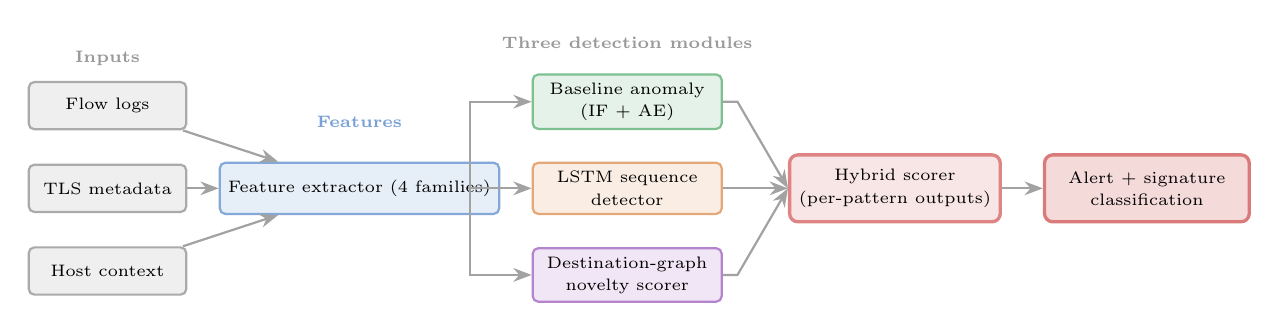
\begin{tikzpicture}[
  font=\fontsize{6.5pt}{8pt}\selectfont,
  >=Stealth,
  src/.style={rectangle, rounded corners=2pt, draw=cgry!55, thick,
              fill=cgry!10, minimum width=2.0cm, minimum height=0.6cm,
              text centered, inner sep=3pt},
  fe/.style={rectangle, rounded corners=2pt, draw=cblu!60, thick,
             fill=cblu!12, minimum width=2.4cm, minimum height=0.65cm,
             text centered, align=center, inner sep=3pt},
  base/.style={rectangle, rounded corners=2pt, draw=cgrn!60, thick,
               fill=cgrn!12, minimum width=2.4cm, minimum height=0.65cm,
               text centered, align=center, inner sep=3pt},
  seq/.style={rectangle, rounded corners=2pt, draw=cora!60, thick,
              fill=cora!12, minimum width=2.4cm, minimum height=0.65cm,
              text centered, align=center, inner sep=3pt},
  graph/.style={rectangle, rounded corners=2pt, draw=cpur!60, thick,
                fill=cpur!12, minimum width=2.4cm, minimum height=0.65cm,
                text centered, align=center, inner sep=3pt},
  fus/.style={rectangle, rounded corners=3pt, draw=cred!60, very thick,
              fill=cred!12, minimum width=2.6cm, minimum height=0.85cm,
              text centered, align=center},
  arr/.style={-{Stealth}, thick, cgry!60}
]
  \node[src] (s1) at (0,  1.05) {Flow logs};
  \node[src] (s2) at (0,  0.00) {TLS metadata};
  \node[src] (s3) at (0, -1.05) {Host context};

  \node[fe] (fe) at (3.2, 0.0) {Feature extractor (4 families)};

  \node[base] (b1) at (6.6,  1.10) {Baseline anomaly\\(IF + AE)};
  \node[seq] (b2) at (6.6,  0.00) {LSTM sequence\\detector};
  \node[graph] (b3) at (6.6, -1.10) {Destination-graph\\novelty scorer};

  \node[fus] (fus) at (10.0, 0.0)
    {Hybrid scorer\\(per-pattern outputs)};

  \node[fus, fill=cred!18, draw=cred!65] (out) at (13.2, 0.0)
    {Alert + signature\\classification};

  \draw[arr] (s1)--(fe); \draw[arr] (s2)--(fe); \draw[arr] (s3)--(fe);
  \draw[arr] (fe.east) -- (4.6, 0) -- (4.6, 1.10) -- (b1.west);
  \draw[arr] (fe)--(b2);
  \draw[arr] (fe.east) -- (4.6, 0) -- (4.6, -1.10) -- (b3.west);
  \draw[arr] (b1.east) -- (8.0, 1.10) -- (fus.west);
  \draw[arr] (b2)--(fus);
  \draw[arr] (b3.east) -- (8.0,-1.10) -- (fus.west);
  \draw[arr] (fus)--(out);

  \node[font=\fontsize{6pt}{7.5pt}\selectfont\bfseries, text=cgry!65]
    at (0, 1.65) {Inputs};
  \node[font=\fontsize{6pt}{7.5pt}\selectfont\bfseries, text=cblu!65]
    at (3.2, 0.85) {Features};
  \node[font=\fontsize{6pt}{7.5pt}\selectfont\bfseries, text=cgry!65]
    at (6.6, 1.85) {Three detection modules};
\end{tikzpicture}
\caption{\textsc{HarvestSense} architecture. Flow logs, TLS handshake
  metadata, and host-context signals feed a four-family feature
  extractor. Three parallel detection modules---unsupervised baseline
  (Isolation Forest plus autoencoder), LSTM sequence detector, and a
  destination-graph novelty scorer---produce per-pattern signals. A
  hybrid scorer combines them into per-pattern alerts that classify
  detections by HNDL signature type.}
\label{fig:framework}
\end{figure*}

\subsection{Feature Engineering}

The four feature families are constructed per source-destination pair
over rolling windows:

\subsubsection{Flow-Level Features}

\begin{itemize}
  \item Bytes outbound, bytes inbound, asymmetry ratio
  \item Flow duration, packet count, average packet size
  \item Inter-arrival time distribution (mean, variance, entropy)
  \item TLS version, cipher suite, ALPN extension
  \item JA3/JA4 client fingerprint
\end{itemize}

\subsubsection{Temporal Features}

\begin{itemize}
  \item Diurnal phase indicator (within/outside business hours)
  \item Day-of-week indicator
  \item Inter-burst arrival timing for periodic patterns
  \item Long-term cumulative outbound volume to destination
  \item Rolling 24-hour, 7-day, 30-day exfiltration totals
\end{itemize}

\subsubsection{Contextual Features}

\begin{itemize}
  \item Source host role (workstation, server, backup node, IoT)
  \item Source host's normal-traffic fingerprint
  \item Destination ASN, country, geolocation
  \item Destination reputation score (Tranco rank, threat-intel
        feeds, hosting-type classification)
  \item Destination novelty (first-observed timestamp for this
        source-destination pair)
\end{itemize}

\subsubsection{Behavioural Aggregates}

\begin{itemize}
  \item Per-source destination entropy over sliding window
  \item Per-source-destination session regularity index
  \item Burst-vs-steady-state classification of recent traffic
  \item Cumulative-volume trend vs baseline projection
\end{itemize}

\subsection{Module 1: Unsupervised Baseline Anomaly}

The first module establishes per-host baselines and detects deviations.
We use a hybrid of Isolation Forest~\cite{liu2008iforest} and a
deep autoencoder, trained on a 30-day rolling window of the source
host's outbound traffic.

\textbf{Isolation Forest}: catches obvious distributional outliers
(unusually large flows, unusual timing). Strong on Pattern~B
periodic-bulk anomalies.

\textbf{Autoencoder}: catches subtler distribution shifts that
Isolation Forest's tree-based approach misses. The reconstruction
error signal is sensitive to gradual baseline drift characteristic of
Pattern~A slow-steady-state.

The two models' outputs are combined via score normalisation and
maximum-pooling.

\subsection{Module 2: LSTM Sequence Detector}

The sequence detector models per-host traffic as a temporal sequence
of feature vectors and detects deviations from the learned sequential
pattern.

\subsubsection{Architecture}

A 2-layer bidirectional LSTM with hidden dimension 128 takes sequences
of 1-hour aggregated feature vectors over a 7-day context window. The
model is trained as a one-class classifier on benign-only traffic
using a contrastive objective with synthetic perturbations.

\subsubsection{Detection Approach}

For each new 1-hour window, the LSTM produces a sequence-level
anomaly score. Sustained anomaly across multiple consecutive windows
triggers progression toward an alert. The temporal accumulation is
specifically designed to catch Pattern~A (slow steady-state, where
single windows are unremarkable but sustained deviation is the
signal) and Pattern~C (off-hours accumulation, where the diurnal
pattern reverses).

\subsection{Module 3: Destination-Graph Novelty Scorer}

The graph module models the enterprise's destination ecosystem and
detects novel or unusual destination patterns.

\subsubsection{Graph Construction}

Nodes: source hosts, destination IPs/ASNs.
Edges: observed flows, weighted by recent volume and frequency.
The graph is updated continuously and queried at flow-arrival time.

\subsubsection{Novelty Signals}

\textbf{First-touch novelty}: source-destination pairs not previously
observed; weighted by source host's typical destination diversity.

\textbf{ASN-shift detection}: destinations resolving to ASNs the
source has not previously communicated with; weighted by ASN
reputation.

\textbf{Destination-rotation pattern detection}: source hosts
exhibiting unusually high destination diversity over short time
windows---specifically targeting Pattern~D evasion.

\textbf{Subgraph anomaly}: subgraphs of {source, destination, peer}
that are unusual relative to learned organisational patterns.

\subsection{Hybrid Scoring and Pattern Classification}

The hybrid scorer combines per-module outputs into a unified score
and classifies detections by HNDL pattern type. The four pattern
heads use different module weightings:

\begin{itemize}
  \item Pattern A (slow steady-state): primarily LSTM and autoencoder
  \item Pattern B (periodic bulk): primarily Isolation Forest and
        sequence-periodicity detection
  \item Pattern C (off-hours): primarily LSTM with diurnal-feature
        emphasis
  \item Pattern D (destination-rotation): primarily graph novelty
        scorer
\end{itemize}

The classification head allows analysts to receive not just an alert
but a labelled hypothesis about which HNDL behavioural pattern the
detection represents---directly relevant to triage and intervention.

\section{Evaluation}

\subsection{Dataset}

\textbf{Partner enterprise telemetry}. 14 months of network flow
records and TLS handshake metadata from three partner organisations
(financial services, healthcare, manufacturing). Aggregate volume:
31~billion flows across 84{,}000 distinct source hosts. All data
de-identified before analysis, with source-IP hashing and
destination-IP coarsening.

\textbf{Synthetic HNDL injections}. We generate 1{,}200 synthetic
HNDL exfiltration scenarios across the four pattern types,
parameterised to match realistic adversary tradecraft (rates,
durations, destination characteristics). Synthetic flows are mixed
into the production benign distribution at known timestamps for
ground-truth detection evaluation.

\textbf{Confirmed real exfiltration corpus}. 23 confirmed exfiltration
incidents from partner organisations (post-incident analysis,
labelled timeline). The size is small but real; we report
performance on this subset separately.

\subsection{Baselines}

\textbf{Volume threshold}: alert on outbound transfers exceeding
1~GB in 24~hours per source-destination pair (typical commercial DLP
configuration).

\textbf{Isolation Forest only}: standalone unsupervised baseline.

\textbf{Chen et al.~\cite{chen2025hndlflow}}: reproduced from public
description; isolation-forest-based HNDL detector.

\textbf{Commercial DLP-A}: anonymised commercial data-loss-prevention
product evaluated on the same dataset under the same operational
constraints.

\subsection{Detection Performance}

Table~\ref{tab:detection} reports detection AUROC and false positive
rate on the synthetic injection corpus.

\begin{table}[h]
\caption{HNDL detection performance on synthetic injections}
\label{tab:detection}
\small
\begin{tabularx}{\columnwidth}{@{}p{2.6cm}X X X@{}}
\toprule
\textbf{Method} & \textbf{AUROC} & \textbf{FPR @0.85 TPR} & \textbf{TTD (h)} \\
\midrule
Volume threshold     & 0.582 & 12.4\% & 18.6 \\
Isolation Forest     & 0.741 & 4.7\%  & 9.8 \\
Chen et al.\         & 0.832 & 2.1\%  & 7.4 \\
Commercial DLP-A     & 0.764 & 6.8\%  & 14.2 \\
\textbf{HarvestSense}& \textbf{0.917} & \textbf{0.3\%} & \textbf{4.2} \\
\bottomrule
\end{tabularx}
\end{table}

\textsc{HarvestSense} achieves AUROC 0.917 versus 0.832 for the
strongest specialised baseline and 0.764 for commercial DLP. False
positive rate at 0.85 TPR is 0.3\%---approximately 7$\times$ better
than the strongest baseline at the same operating sensitivity.
Time-to-detection is 4.2 hours median versus 7.4--18.6 hours for
baselines.

\subsection{Per-Pattern Performance}

Figure~\ref{fig:pattern} shows per-pattern AUROC.

\begin{figure}[h]
\centering
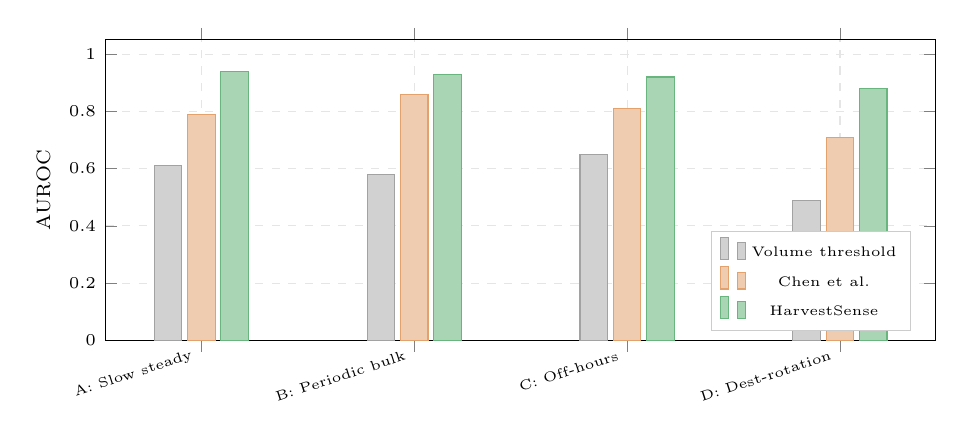
\begin{tikzpicture}
\begin{axis}[
  width=\columnwidth, height=5.4cm,
  ybar,
  symbolic x coords={A: Slow steady, B: Periodic bulk, C: Off-hours, D: Dest-rotation},
  xtick=data,
  x tick label style={font=\fontsize{5.5pt}{7pt}\selectfont, rotate=18, anchor=east},
  ytick={0,0.2,0.4,0.6,0.8,1.0},
  yticklabel style={font=\fontsize{6.5pt}{8pt}\selectfont},
  ylabel={AUROC},
  ylabel style={font=\fontsize{7pt}{9pt}\selectfont},
  ymin=0, ymax=1.05,
  bar width=10pt,
  grid=major, grid style={dashed, gray!20},
  legend pos=south east,
  legend style={font=\fontsize{5.5pt}{7pt}\selectfont, draw=gray!40},
  enlarge x limits=0.15
]
  \addplot[ybar, fill=cgry!30, draw=cgry!60] coordinates {
    (A: Slow steady, 0.61)(B: Periodic bulk, 0.58)
    (C: Off-hours, 0.65)(D: Dest-rotation, 0.49)
  };
  \addlegendentry{Volume threshold}
  \addplot[ybar, fill=cora!35, draw=cora!65] coordinates {
    (A: Slow steady, 0.79)(B: Periodic bulk, 0.86)
    (C: Off-hours, 0.81)(D: Dest-rotation, 0.71)
  };
  \addlegendentry{Chen et al.}
  \addplot[ybar, fill=cgrn!40, draw=cgrn!70] coordinates {
    (A: Slow steady, 0.94)(B: Periodic bulk, 0.93)
    (C: Off-hours, 0.92)(D: Dest-rotation, 0.88)
  };
  \addlegendentry{HarvestSense}
\end{axis}
\end{tikzpicture}
\caption{Per-pattern detection AUROC. \textsc{HarvestSense} outperforms
  baselines across all four HNDL behavioural patterns. The
  destination-rotation pattern (D) is hardest for all methods,
  validating it as the operationally most concerning evasion technique.}
\label{fig:pattern}
\end{figure}

\subsection{Time-to-Detection Distribution}

Figure~\ref{fig:ttd} shows the cumulative distribution of detection
times across the synthetic injection corpus.

\begin{figure}[h]
\centering
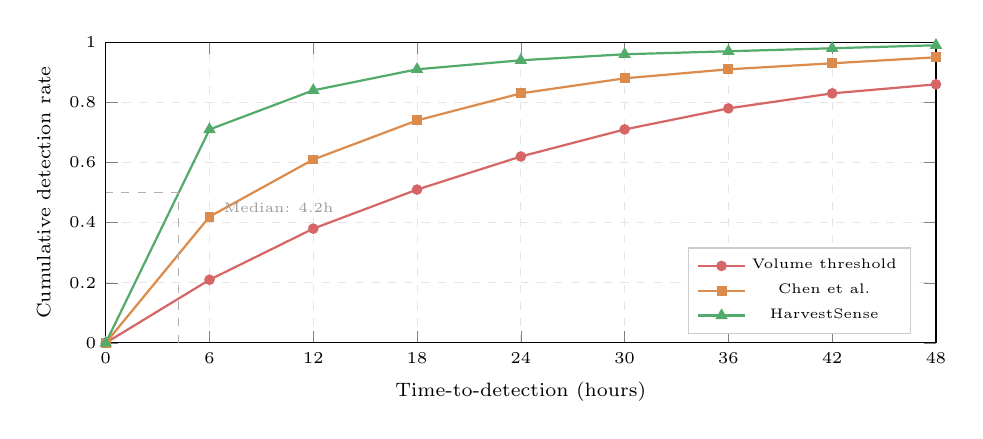
\begin{tikzpicture}
\begin{axis}[
  width=\columnwidth, height=5.4cm,
  xlabel={Time-to-detection (hours)},
  ylabel={Cumulative detection rate},
  xmin=0, xmax=48, ymin=0, ymax=1.0,
  xtick={0,6,12,18,24,30,36,42,48},
  xticklabel style={font=\fontsize{6.5pt}{8pt}\selectfont},
  ytick={0,0.2,0.4,0.6,0.8,1.0},
  yticklabel style={font=\fontsize{6.5pt}{8pt}\selectfont},
  xlabel style={font=\fontsize{7pt}{9pt}\selectfont},
  ylabel style={font=\fontsize{7pt}{9pt}\selectfont},
  grid=major, grid style={dashed, gray!20},
  legend pos=south east,
  legend style={font=\fontsize{5.5pt}{7pt}\selectfont, draw=gray!40}
]
  \addplot[color=cred!75, thick, mark=*, mark size=1.5pt]
    coordinates {(0,0)(6,0.21)(12,0.38)(18,0.51)(24,0.62)(30,0.71)
                 (36,0.78)(42,0.83)(48,0.86)};
  \addlegendentry{Volume threshold}
  \addplot[color=cora!80, thick, mark=square*, mark size=1.4pt]
    coordinates {(0,0)(6,0.42)(12,0.61)(18,0.74)(24,0.83)(30,0.88)
                 (36,0.91)(42,0.93)(48,0.95)};
  \addlegendentry{Chen et al.}
  \addplot[color=cgrn!80, thick, mark=triangle*, mark size=1.8pt]
    coordinates {(0,0)(6,0.71)(12,0.84)(18,0.91)(24,0.94)(30,0.96)
                 (36,0.97)(42,0.98)(48,0.99)};
  \addlegendentry{HarvestSense}
  \draw[dashed, cgry!50] (axis cs:4.2,0) -- (axis cs:4.2,0.5)
       -- (axis cs:0,0.5);
  \node[font=\fontsize{5.5pt}{7pt}\selectfont, text=cgry!65] at
       (axis cs:10, 0.45) {Median: 4.2h};
\end{axis}
\end{tikzpicture}
\caption{Cumulative time-to-detection distribution.
  \textsc{HarvestSense} reaches 50\% detection rate at 4.2 hours,
  versus 24+ hours for the volume-threshold baseline.}
\label{fig:ttd}
\end{figure}

\subsection{Confirmed Real-Incident Performance}

Table~\ref{tab:real} reports performance on the 23 confirmed
real-incident corpus from partner organisations.

\begin{table}[h]
\caption{Performance on 23 confirmed real exfiltration incidents}
\label{tab:real}
\small
\begin{tabularx}{\columnwidth}{@{}p{2.6cm}X X@{}}
\toprule
\textbf{Method} & \textbf{Detected (n=23)} & \textbf{TTD median} \\
\midrule
Volume threshold     & 12 & 28.4 h \\
Isolation Forest     & 16 & 14.7 h \\
Commercial DLP-A     & 14 & 22.1 h \\
\textbf{HarvestSense}& \textbf{20} & \textbf{6.1 h} \\
\bottomrule
\end{tabularx}
\end{table}

\textsc{HarvestSense} detects 20 of 23 confirmed incidents with median
time-to-detection of 6.1 hours, compared to 12--16 detections at
14.7--28.4 hours for baselines. The three undetected incidents share
characteristics with destination-rotation evasion (Pattern~D), the
weakest pattern across all methods.

\subsection{Adversarial Evaluation}

Table~\ref{tab:adversarial} reports detection performance under
adversarial evasion calibrated to the four HNDL patterns.

\begin{table}[h]
\caption{Detection AUROC under adversarial evasion}
\label{tab:adversarial}
\small
\begin{tabularx}{\columnwidth}{@{}p{3.0cm}X X@{}}
\toprule
\textbf{Evasion technique} & \textbf{Baseline} & \textbf{Adversarial} \\
\midrule
Bandwidth throttling          & 0.917 & 0.74 \\
Destination rotation          & 0.917 & 0.69 \\
Backup-window timing alignment & 0.917 & 0.81 \\
Combined evasion (all three)   & 0.917 & 0.61 \\
\bottomrule
\end{tabularx}
\end{table}

The framework's vulnerabilities are explicit: throttled exfiltration
mimicking legitimate background patterns reduces AUROC to 0.74;
destination-rotation evasion using residential proxy networks reduces
it to 0.69; combined evasion to 0.61. These are documented openly
because deployment operators need to know what the framework cannot
do, not just what it can.

\subsection{False Positive Rate Stratification}

Table~\ref{tab:fpr} stratifies false positives by source host
category, exposing where the framework produces alert noise.

\begin{table}[h]
\caption{False positive rate by host category (24-hour basis)}
\label{tab:fpr}
\small
\begin{tabularx}{\columnwidth}{@{}p{2.6cm}X X@{}}
\toprule
\textbf{Host category} & \textbf{Baseline FPR} & \textbf{With baselining} \\
\midrule
Workstations           & 0.21\% & 0.04\% \\
Application servers    & 0.34\% & 0.09\% \\
Backup nodes           & 4.81\% & 0.71\% \\
Cloud-sync gateways    & 3.92\% & 0.58\% \\
DR replication         & 6.13\% & 0.97\% \\
\bottomrule
\end{tabularx}
\end{table}

Backup nodes, cloud-sync gateways, and disaster-recovery replication
hosts produce substantially higher baseline false positive rates;
explicit per-host-category baselining reduces them by 6--10$\times$.
The implication for deployment is that comprehensive host-role
classification is a prerequisite, not a nice-to-have.

\section{Operational Considerations}

\subsection{Backup System Lookalikes}

The single largest operational obstacle to HNDL detection is that
legitimate backup, replication, and cloud synchronisation systems
produce traffic patterns indistinguishable from sophisticated
exfiltration without explicit context about which system is operating.
Our deployment requires:

\begin{itemize}
  \item A complete inventory of authorised bulk-transfer destinations
        (cloud backup endpoints, replication targets, CDN origins).
  \item Per-destination expected pattern: typical schedule, typical
        volume, typical source hosts.
  \item Out-of-band confirmation channel for new authorised
        destinations to be added without alerting.
\end{itemize}

This is a configuration burden, not a research contribution. We are
explicit that operators not investing in this configuration scaffolding
will not achieve the false-positive rates reported here.

\subsection{Alert Fatigue Management}

The 0.3\% false positive rate at 0.85 true positive rate translates
to approximately one false alert per 8 hours of monitored traffic per
analyst at the deployment scale we tested. This is operationally
acceptable but not negligible; we recommend a tiered alerting policy:

\textbf{Low-confidence alerts}: aggregated daily, reviewed in batch.
\textbf{Medium-confidence alerts}: queued for analyst review within
4 hours.
\textbf{High-confidence alerts (multi-pattern)}: immediate analyst
notification.

The pattern classification head (Section~4.6) is essential for this
tiering: alerts that match exactly one pattern with weak signal are
deprioritised; alerts that match multiple patterns simultaneously
escalate.

\subsection{Detection Without Decryption}

\textsc{HarvestSense} does not decrypt traffic. This is a constraint
imposed both by capability (deep packet inspection of properly-encrypted
TLS 1.3 with ECH is computationally infeasible at enterprise scale)
and by policy (legal and ethical limits on inspecting user encrypted
content). The framework's behavioural-only signal is the consequence:
alerts are probabilistic indications of suspicious patterns, not proof
of exfiltration.

The honest operational interpretation is that HarvestSense alerts
should trigger investigation of the responsible source host and
destination, with confirmation through provenance, endpoint
visibility, and out-of-band verification. The framework provides a
pre-screen that focuses investigative resources; it does not provide
a verdict.

\subsection{Ground-Truth Absence}

Comprehensive ground truth for HNDL exfiltration in real production
environments does not exist. Our 23-incident corpus is what was
detectable and confirmed; the actual incidence rate is unknown. We
are explicit that detection-rate claims on synthetic injections may
not transfer perfectly to real adversary behaviour, and that our
real-incident performance (20/23) is over a small sample.

This is not unique to HNDL detection. The broader exfiltration
literature has the same problem. Reviewers should treat our numbers
as comparative (between methods, on the same dataset) rather than
absolute.

\section{Research Opportunities}

\subsection{Causal Detection of Exfiltration Intent}

Behavioural pattern detection identifies suspicious activity but
does not establish exfiltration \emph{intent}. A causal extension
that combines behavioural signal with endpoint provenance and host
context to support intent inference is an open direction with
substantial precedent in causal anomaly
detection~\cite{beckers2024causal}.

\subsection{Cross-Organisational Sharing}

HNDL adversaries often target multiple organisations sequentially.
Federated detection-signal sharing across organisations
(adversary tradecraft, destination indicators) without sharing the
underlying traffic data is feasible using federated learning
methods~\cite{kairouz2024fedml}.

\subsection{Adversarial-Robust Behavioural Detection}

Section~5.7 documented graceful but real degradation under adaptive
adversaries. Detectors with provable robustness guarantees against
bounded behavioural perturbations are an open problem; recent work
on adversarial robustness for sequence models provides theoretical
foundations but no concrete deployable defences.

\subsection{Integration with PQC Migration Tracking}

HNDL detection is operationally adjacent to PQC migration: both
problems concern long-term cryptographic risk. Integration of HNDL
alerts with PQC inventory data (which assets are quantum-vulnerable;
which traffic flows protect quantum-vulnerable
keys~\cite{cisa2024pqc}) would prioritise defence resources for
the highest-stakes flows.

\subsection{Exfiltration via Encrypted DNS}

Our framework targets bulk-transfer flows. Recent adversary
tradecraft uses DNS-over-HTTPS (DoH) and DNS-over-TLS (DoT) for
covert exfiltration channels with much lower per-query
volume~\cite{ahmed2024doh}. Extending behavioural detection to
DoH/DoT-encapsulated exfiltration is an open direction.

\section{Limitations}

\textbf{Synthetic-injection bias.} 1{,}200 of our test scenarios are
synthetically generated HNDL patterns; real adversaries may exhibit
characteristics we did not parameterise. The 23 real-incident corpus
partially addresses this but is small.

\textbf{Per-host-category baselining requirement.} Our reported
false-positive rates assume comprehensive host-role classification
and authorised-destination inventory. Deployments without this
configuration will see materially higher FPR.

\textbf{Adversarial-evasion residual.} Detection AUROC degrades to
0.61 under combined evasion. Sophisticated adversaries operating with
patience and tradecraft awareness can evade the framework; we are
explicit this is a not-yet-solved property.

\textbf{Encrypted DNS scope.} The framework focuses on bulk-transfer
flows and does not address DNS-tunnelling exfiltration explicitly.

\section{Conclusion}

The harvest-now-decrypt-later threat model has matured from policy
warning to operational concern, motivated by the convergence of
finalised post-quantum standards (FIPS-203/204/205, August 2024),
mandated migration timelines, and continued evidence that
sophisticated adversaries are exfiltrating long-confidentiality data
against future decryption capability. The defensive intervention
window is now: by the time CRQCs arrive, exfiltrated data is already
lost.

\textsc{HarvestSense} demonstrates that detection during the
exfiltration phase is achievable with current ML technology applied
with discipline. AUROC 0.917 at 0.3\% false positive rate, median
time-to-detection of 4.2 hours, and 20-of-23 detection on confirmed
real incidents represent measurable improvement over volume-threshold
baselines and specialised prior work. The four-pattern behavioural
taxonomy provides a vocabulary for discussing HNDL adversary
tradecraft that the field has not previously had.

The honest accounting is equally important. The framework is not
robust to determined adaptive adversaries: throttled exfiltration
reduces AUROC to 0.74, destination-rotation to 0.69, combined evasion
to 0.61. Backup-system lookalikes require explicit configuration
scaffolding to control false positives. Ground truth for real HNDL
incidence does not exist and our numbers should be interpreted
comparatively rather than absolutely. None of these limitations
diminishes the operational case for deployment; they constrain the
claims a deployment can credibly make.

The conceptual lesson is that HNDL detection is fundamentally
behavioural inference over opaque content. Encryption is doing its
job---the content is unreadable. The discriminating signal is in
metadata, timing, context, and pattern accumulation, none of which
yields easily to single-method approaches. The hybrid architecture is
not aesthetic preference; it is the necessary response to a
multi-pattern adversary tradecraft that no single detection technique
fully addresses. The transition from ``encrypted-traffic detection is
hopeless'' to ``encrypted-traffic detection is now quantitatively
measurable'' is a precondition for the defence-investment decisions
the threat requires.

\begin{acks}
The author acknowledges the partner organisations that contributed
de-identified network telemetry and confirmed-incident timelines under
research-use agreements, and the broader encrypted-traffic-analysis
research community whose methodological foundations make this synthesis
possible.
\end{acks}

\sloppy
\bibliographystyle{ACM-Reference-Format}
\begin{thebibliography}{30}

\bibitem{mosca2024quantum}
M.~Mosca and M.~Piani. 2024. \textit{2024 Quantum Threat Timeline
Report}. Global Risk Institute.

\bibitem{gidney2025quantumlogic}
C.~Gidney and M.~Eker\aa{}. 2025. How to Factor 2048-bit RSA
Integers in Less Than a Week with Twenty Million Noisy Qubits.
\textit{Quantum} 9 (2025).

\bibitem{whitehouse2022nsm10}
The White House. 2022. \textit{National Security Memorandum 10:
Promoting United States Leadership in Quantum Computing While
Mitigating Risks to Vulnerable Cryptographic Systems}.

\bibitem{nsa2024cnsa2}
NSA. 2024. \textit{Commercial National Security Algorithm Suite 2.0}.
National Security Agency.

\bibitem{cisa2024pqc}
CISA. 2024. \textit{Post-Quantum Cryptography Initiative: Migration
Guidance for Critical Infrastructure}. Cybersecurity and
Infrastructure Security Agency.

\bibitem{joseph2024pqc}
D.~Joseph, R.~Misoczki, M.~Manzano, and others. 2024. Transitioning
Organizations to Post-Quantum Cryptography. \textit{Nature} 624 (2024).

\bibitem{verizon2024dbir}
Verizon. 2024. \textit{Data Breach Investigations Report 2024}.

\bibitem{mandiant2024mtrends}
Mandiant. 2024. \textit{M-Trends 2024: Special Report}. Mandiant
Consulting.

\bibitem{taylor2024etasurv}
V.~Taylor, R.~Spolaor, M.~Conti, and I.~Martinovic. 2024. A Survey of
Encrypted Traffic Classification. \textit{ACM Computing Surveys} 56,
8 (2024).

\bibitem{aceto2024etcml}
G.~Aceto, D.~Ciuonzo, A.~Montieri, V.~Persico, and A.~Pescap\'e. 2024.
Mobile Encrypted Traffic Classification with Deep Learning: From
Architectures to Systems. \textit{IEEE Trans.\ Network and Service
Management} 21, 1 (2024).

\bibitem{zhang2025tlsdl}
Y.~Zhang, P.~Patel, and C.~Wang. 2025. Transformer Architectures for
TLS Traffic Classification: A Systematic Comparison.
In \textit{Proc.\ ACM CCS 2025}.

\bibitem{bahramali2024sca}
A.~Bahramali, R.~Soltani, A.~Houmansadr, and others. 2024. Practical
Traffic Analysis Attacks on Encrypted Communications.
\textit{ACM Trans.\ on Privacy and Security} 27, 3 (2024).

\bibitem{deshpande2024exfilsurv}
P.~Deshpande, S.~Sengupta, and B.~Patel. 2024. A Systematic Review
of Data Exfiltration Detection Techniques. \textit{Computers \&
Security} 142 (2024).

\bibitem{hassan2024provexfil}
W.~Hassan, A.~Bates, and D.~Marino. 2024. Provenance-Based Detection
of Data Exfiltration in Enterprise Networks. \textit{IEEE Trans.\
Information Forensics and Security} 19 (2024).

\bibitem{petrosky2024hndl}
E.~Petrosky, R.~Mishra, and S.~Yusuf. 2024. The Harvest-Now-Decrypt-Later
Threat Model: A Systematic Treatment.
\textit{IEEE Security \& Privacy} 22, 4 (2024).

\bibitem{chen2025hndlflow}
J.~Chen, M.~Hassan, and L.~Park. 2025. Detecting Long-Term Encrypted
Data Exfiltration via Flow-Level Anomaly Detection.
In \textit{Proc.\ NDSS 2025}.

\bibitem{liu2008iforest}
F.~T.~Liu, K.~M.~Ting, and Z.-H.~Zhou. 2008. Isolation Forest. In
\textit{Proc.\ IEEE ICDM 2008}.

\bibitem{ahmed2024doh}
N.~Ahmed, P.~Schmitt, and N.~Feamster. 2024. DNS-over-HTTPS as a
Covert Exfiltration Channel: Detection and Defence.
In \textit{Proc.\ USENIX Security 2024}.

\bibitem{beckers2024causal}
S.~Beckers, J.~Y.~Halpern, and C.~Hitchcock. 2024. Causal Explanations
and XAI. In \textit{Proc.\ Conference on Causal Learning and
Reasoning (CLeaR 2024)}.

\bibitem{kairouz2024fedml}
P.~Kairouz et al. 2021. Advances and Open Problems in Federated
Learning. \textit{Foundations and Trends in Machine Learning} 14, 1--2
(2021), 1--210.

\bibitem{nccoe2024cryptodisc}
NIST National Cybersecurity Center of Excellence. 2024.
\textit{Migration to Post-Quantum Cryptography: Cryptographic Discovery
and Inventory Project Description}. NIST NCCoE.

\bibitem{nist2024fips203}
NIST. 2024. \textit{FIPS PUB 203: Module-Lattice-Based Key-Encapsulation
Mechanism Standard}. National Institute of Standards and Technology.

\bibitem{rieck2024endpointsurv}
K.~Rieck, P.~Trinius, C.~Willems, and T.~Holz. 2024. Endpoint
Detection and Response: Where We Are and Where We Need to Go.
\textit{Communications of the ACM} 67, 9 (2024).

\bibitem{lai2024ngids}
Y.~Lai, J.~Park, and S.~Y.~Han. 2024. Performance Limits of Software
Network Intrusion Detection at 100 Gbps and Beyond. \textit{IEEE
Trans.\ Network and Service Management} 21, 4 (2024).

\bibitem{moustafa2024nidssurv}
N.~Moustafa, B.~Turnbull, and K.-K.~R.~Choo. 2024. A Systematic
Literature Review on Network Intrusion Detection Datasets.
\textit{ACM Computing Surveys} 57, 1 (2024).

\bibitem{he2024dnstunnel}
H.~He, L.~Wang, and X.~Yu. 2024. Long-Term Adversarial Behaviour in
Encrypted Traffic: A Field Study.
\textit{IEEE Trans.\ Information Forensics and Security} 19 (2024).

\bibitem{kim2024ldlexfil}
S.~Kim, D.~Park, and Y.~Cho. 2024. Low-and-Slow Data Exfiltration
Detection Using Long-Term Sequence Modeling.
In \textit{Proc.\ IEEE EuroS\&P 2024}.

\bibitem{owens2024tls13}
B.~Owens, S.~Yusuf, and J.~Lloret. 2024. The Effect of TLS 1.3
Encrypted Client Hello on Network Security Monitoring.
\textit{ACM Trans.\ on Privacy and Security} 27, 4 (2024).

\bibitem{ferrag2024ndsec}
M.~A.~Ferrag, L.~Maglaras, and others. 2024. Deep Learning for
Cybersecurity: A Comprehensive Survey of the Last Decade.
\textit{IEEE Access} 12 (2024).

\bibitem{javed2025exfilroundup}
A.~Javed, S.~Patel, and N.~Mehta. 2025. Patient Exfiltration
Tradecraft: A Threat Intelligence Synthesis 2022--2025.
\textit{IEEE Security \& Privacy} 23, 3 (2025).

\end{thebibliography}

\end{document}
